% Chapter Template

\chapter{Introduction to Thesis Topic} % Main chapter title

\label{Chapter1} % Change X to a consecutive number; for referencing this chapter elsewhere, use \ref{ChapterX}

\lhead{Chapter 1. \emph{Introduction to Thesis Topic}} % Change X to a consecutive number; this is for the header on each page - perhaps a shortened title

%----------------------------------------------------------------------------------------
%	SECTION 1
%----------------------------------------------------------------------------------------

Data Centers have emerged as the basic unit for providing web services to customers by major technology companies.
They house servers in the thousands and tens of thousands, with servers often serving as backups to ensure reliability.
Traffic in data centers is often organized in a tree like structure, with top of rack switches, aggregate switches and core
switches. The tree like structure is easy to maintain and scale to meet the growing number of clients.
\newline
The reliability of data center network infrastructure is critically important for ensuring seamless user experience.
Companies like Facebook\cite{datacenter} and Google\cite{googleOpenflow} have spent considerable investments into developing frameworks for
automating fault detection and repair of networks. Even so, the nature and distribution of faults in data center networks
isn't completely understood, and many faults like microbursts due to fan-in traffic go undetected. A closer look is needed at the type of faults
that occur in data center networks and on how they can be diagnosed.
\newline
Modern data centres operate at throughputs of close to a few hundreds of Gbps, implying packets coming in at a few hundreds of nanoseconds
apart. Most monitoring solutions offer resolution of the order of milliseconds, and hence are inadequate
for recording and detection of events that last for sub millisecond intervals. This motivates the need for
having a diagnosis system to distinguish events at nanosecond level by leveraging advances in data plane programming\cite{dptp}.
\newline
This thesis aims to discuss techniques for diagnosing faults in data centers, develop a monitoring system to view them, 
at nanosecond resolution. It is also demonstrated that appropriate calculations can be performed on the SQL queries
to extract quantities like ingress throughputs, egress throughputs, relative ratios of packets in a network, (all at nanosecond
resolution) thereby demonstrating that collecting relational data about switches is a simple and yet powerful way to extract meaningful 
data and create relevant visualizations\cite{grafana} which can help a network administrator determine the root cause of faults in the network 
and address them.

A high level architecture diagram of the proposition is shown in Figure \ref{fig:Architecture Diagram}

\begin{figure}[htbp]
	\centering
		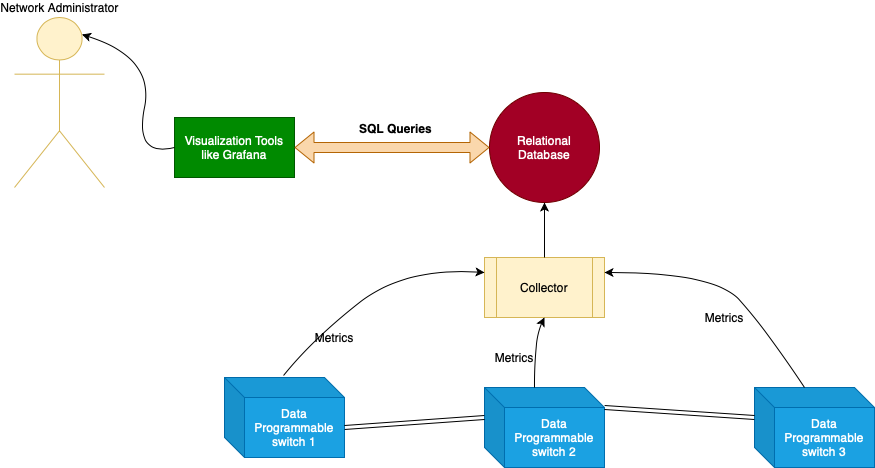
\includegraphics[width=1.0\columnwidth]{Figures/ArchitectureDiagram.png}
		\rule{35em}{0.5pt}
	\caption[Architecture Diagram]{Architecture Diagram of proposed system}
	\label{fig:Architecture Diagram}
\end{figure}